\subsubsection{全体像}
本実験で用いる学習データセット$\datasetTrain$を
\begin{equation}
    \datasetTrain = \lrc{\lr{\video, \spWaveformGt, \spkEmb, \melGt, \hubertIntGt, \hubertDiscGt}}_{\numLower = 1}^{\numUpper}
\end{equation}
とする.各$\numLower$に対し,$\video \in \videoSet$は口唇動画, $\spWaveformGt \in \spWaveformSet$は原音声の音声波形,$\spkEmb \in \spkEmbSet$は話者埋め込みベクトル,$\melGt \in \melSet$はメルスペクトログラム,$\hubertIntGt \in \hubertIntSet$はHuBERT中間特徴量,$\hubertDiscGt \in \hubertDiscGtSet$はHuBERT離散特徴量とする.ここで,話者埋め込めベクトル$\spkEmb$は,事前学習済みの話者識別モデル\cite{wan2018generalized}を利用して得られた音声の話者性を反映するベクトルであり,
\begin{equation}
    \spkEmb = \frac{1}{|\mathcal{\indexUpper}|} \sum_{\indexLower \in \mathcal{\indexUpper}} \spkEmbExtractor\lr{\bm{\outputLower}^{\text{sp-wf}}_{\indexLower}; \weightSpk}
\end{equation}
で与えられる.$\mathcal{\indexUpper}$は学習データセット$\datasetTrain$において、話者$s_{n}$と話者が同一であるデータのインデックス集合から、ランダムに$\numUpper_{\text{spk-emb}}$個のインデックスを抽出した部分集合とする。すなわち、
\begin{equation}
    \mathcal{\indexUpper} \subseteq \{\indexLower \mid \indexLower \in \{1, \ldots, N\}, ~ s_{\indexLower} = \spkId\}, \quad |\mathcal{\indexUpper}| = \numUpper_{\text{spk-emb}}
\end{equation}
である。次に,HuBERT中間特徴量とHuBERT離散特徴量は,HuBERTにおける畳み込みエンコーダまで(Transformer層以前)を$\hubertConv$,HuBERTにおけるTransformer層($\hubertConv$以後)を$\hubertTransformer$,k-means法を$\kmeans$,インデックス系列をOne-hotベクトルに変換する関数を$\onehot$とすると,
\begin{gather}
    \hubertIntGt = \hubertConv\lr{\spWaveformGt; \weightHuBERT} \\
    \hubertDiscGt = \onehot\lr{\kmeans\lr{\hubertTransformer\lr{\hubertIntGt; \weightHuBERT}}}
\end{gather}
で与えられる.ここで,$\weightHuBERT$はHuBERTの事前学習済み重みを表し,$\hubertConv, \hubertTransformer$にこの重みを読み込んで処理したことを意味する.$\kmeans$は本実験の主な検討対象であるDNNではないため,ここでは単にクラスタリングを行う関数として表記した.図\ref{sec4:fig:hubert}に、HuBERTを利用した特徴量計算の流れを示す。以上の処理は,すべてモデルの学習を開始する以前に計算されているものとする.

\begin{figure}[b]
    \centering
    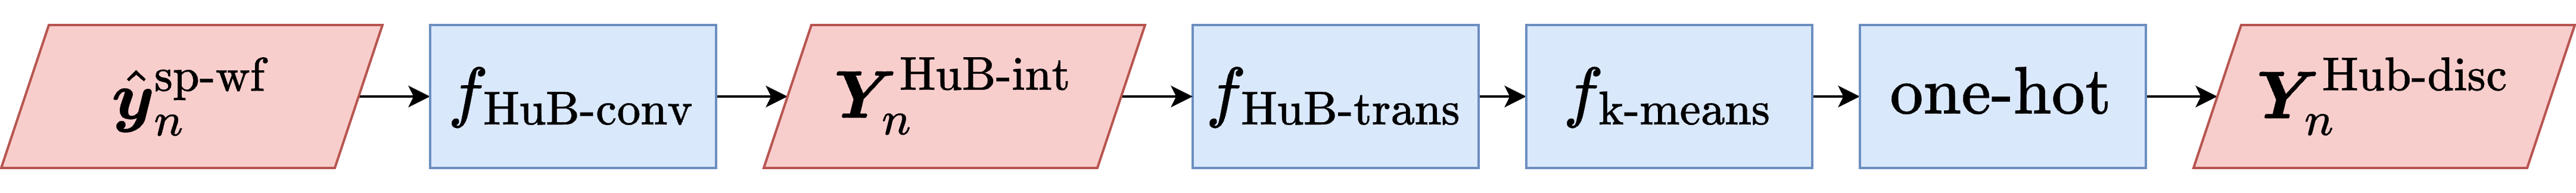
\includegraphics[height=12mm]{./figure/sec4/model_2/hubert.drawio.png}
    \caption{HuBERT}
    \label{sec4:fig:hubert}
\end{figure}

提案手法を図\ref{sec4:fig:overview}に示す.提案手法は,ネットワークA,ネットワークB,ボコーダの三つからなる.まず,ネットワークAを$\myNetworkA$とすると,$\myNetworkA$の行う処理は,
\begin{equation}
    \label{sec4:eq:networkA_overview}
    \hubertIntPred, \melPredA, \hubertDiscPredA = \myNetworkA\lr{\video, \spkEmb; \weightA}
\end{equation}
と表される.ここで,$\hubertIntPred \in \hubertIntSet$は予測HuBERT中間特徴量,$\melPredA \in \melSet$はネットワークAの予測メルスペクトログラム,$\hubertDiscPredA \in \hubertDiscPredSet$はネットワークAのHuBERT離散特徴量に対するロジットを表す.次に,ネットワークBを$\myNetworkB$とすると,$\myNetworkB$の行う処理は,
\begin{equation}
    \melPredB, \hubertDiscPredB = \myNetworkB\lr{\hubertIntPred, \spkEmb; \weightB}
\end{equation}
と表される.ここで,$\melPredB \in \melSet$はネットワークBの予測メルスペクトログラム,$\hubertDiscPredB \in \hubertDiscPredSet$はネットワークBのHuBERT離散特徴量に対するロジットを表す.最後に,音声波形を生成するボコーダを$\vocoder$とすると,$\vocoder$の行う処理は,
\begin{equation}
    \spWaveformPred = \vocoder\lr{\melPredB, \hubertDiscPredB}
\end{equation}
と表される.まとめると,提案手法は口唇動画と話者埋め込みベクトルを入力とし,ネットワークAとネットワークBによって中間表現を獲得後,中間表現をボコーダに入力することで音声波形を生成するものである.

\begin{figure}[bt]
    \centering
    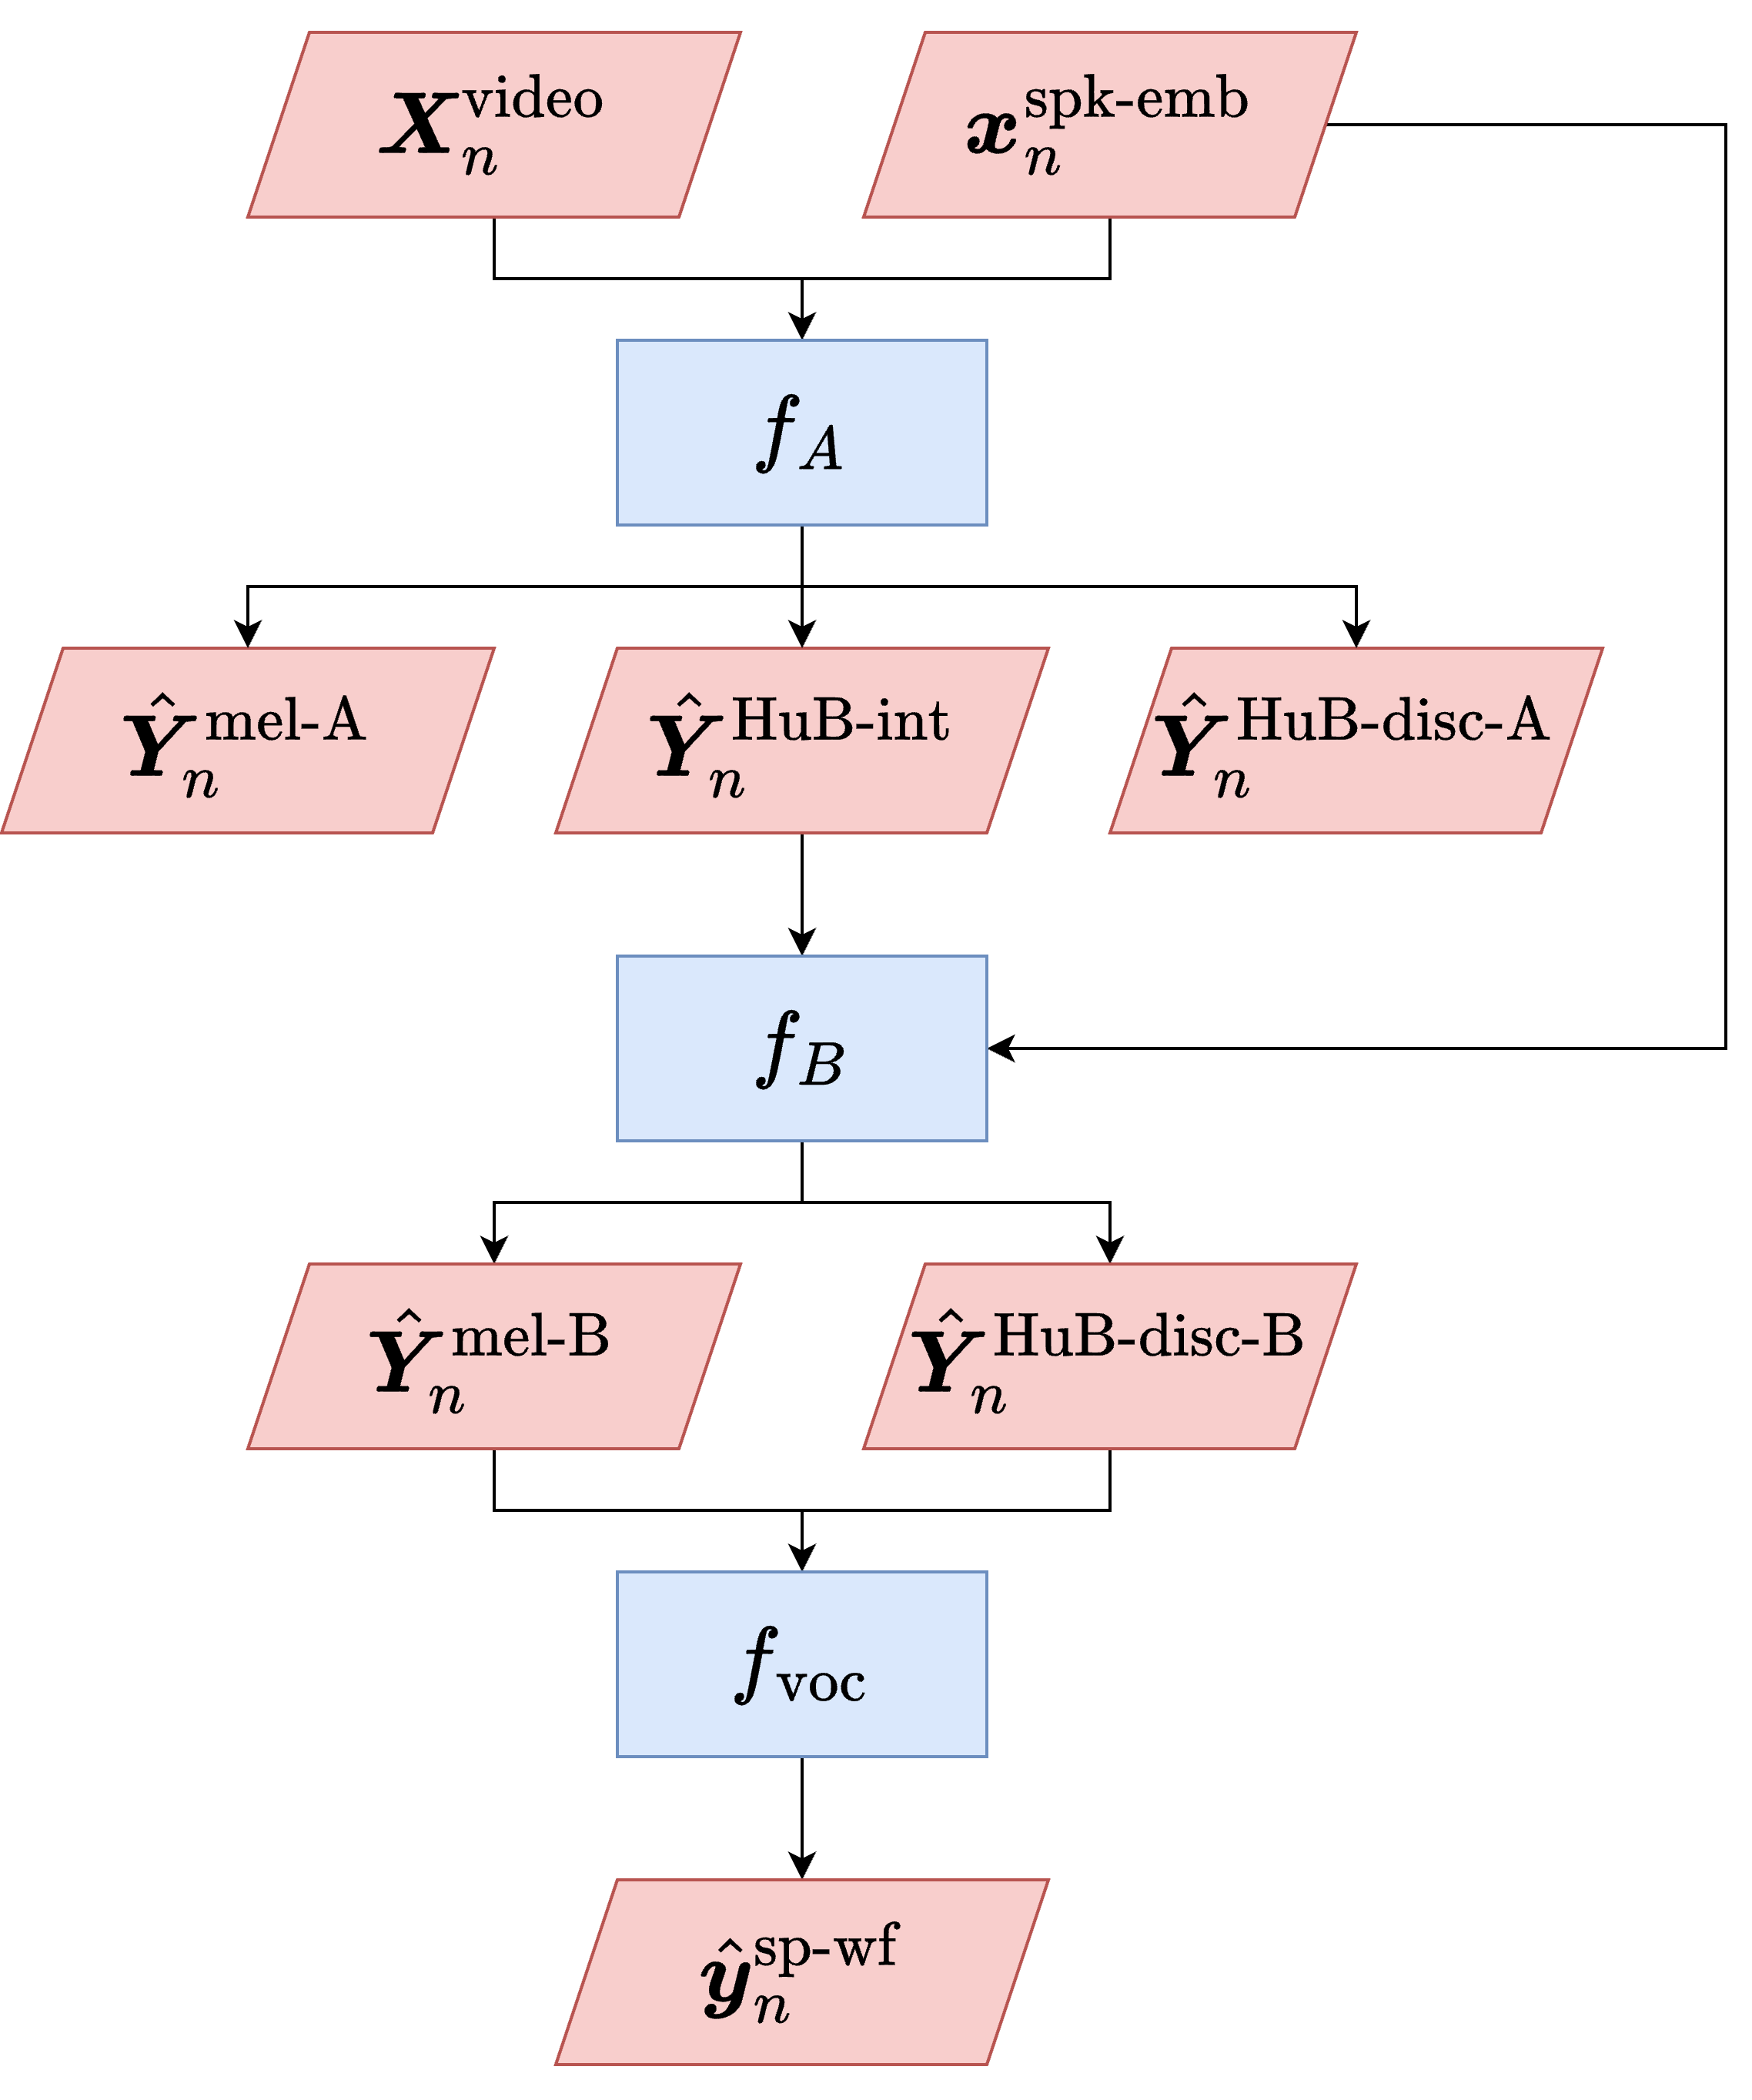
\includegraphics[height=100mm]{./figure/sec4/model_2/overview.drawio.png}
    \caption{提案手法の全体像}
    \label{sec4:fig:overview}
\end{figure}

\subsubsection{ネットワークA}
ネットワークAを図\ref{sec4:fig:networkA}に示す。ネットワークAでは,まず,口唇動画$\video$をAVHuBERTに通すことで,特徴量$\featureA \in \featureASet$に変換する.これは,
\begin{equation}
    \featureA = \AVHuBERT\lr{\video; \weightA}
\end{equation}
と表される.次に,$\featureA$の各時刻$t$におけるベクトルに対し,話者埋め込みベクトル$\spkEmb$を次元方向に結合してから,全結合層によって次元を再度圧縮し,元の次元に戻す.これは,
\begin{equation}
    \featureA = \myNetworkSpkMerge\lr{\concat{\featureA, \lrRepeat{\spkEmb}{T}}; \weightA}
\end{equation}
と表される.次に,話者埋め込みベクトルが統合された特徴量に対する後処理として,$\myNetworkPost$を適用する.これは,
\begin{equation}
    \featureA = \myNetworkPost\lr{\featureA; \weightA}
\end{equation}
と表される.ここで、後処理層$\myNetworkPost$の構造を図\ref{sec4:fig:post}に示す。$\myNetworkPost$は主に一次元畳み込み層と残差結合からなるネットワークである。$\AVHuBERT$はMasked Predictionによって事前学習されたモデルであるから、動画の文脈的な構造を考慮するのに適していると考えられる。一方、音声合成に必要となる話者性は発話に依存しない、すなわち動画の文脈的な構造とは別の性質を持った情報だと考えられる。よって、$\myNetworkPost$は話者埋め込みベクトル$\spkEmb$が次元方向に結合された特徴量$\featureA$に対し、特に話者性を考慮した特徴量の変換を行うために導入した。最後に,$\featureA$を全結合層を通して変換することで,予測対象であるHuBERT中間特徴量,メルスペクトログラム,HuBERT離散特徴量に対するロジットを得る.これは,
\begin{gather}
    \hubertIntPred = \myNetworkFcHubInt\lr{\featureA; \weightA} \\
    \melPredA = \myNetworkFcMel\lr{\featureA; \weightA} \\
    \hubertDiscPredA = \myNetworkFcHubDisc\lr{\featureA; \weightA}
\end{gather}
と表される.

ネットワークAの役割は,続くネットワークBの入力であるHuBERT中間特徴量を予測することである.これに対し,メルスペクトログラムとHuBERT離散特徴量の推定を同時に行った理由は,先行研究\cite{kim2023lip_multitask,choi2023intelligible}においてマルチタスク学習の有効性が確認されており、HuBERT中間特徴量の推定においても有効ではないかと考えたからである。

\begin{figure}[bt]
    \centering
    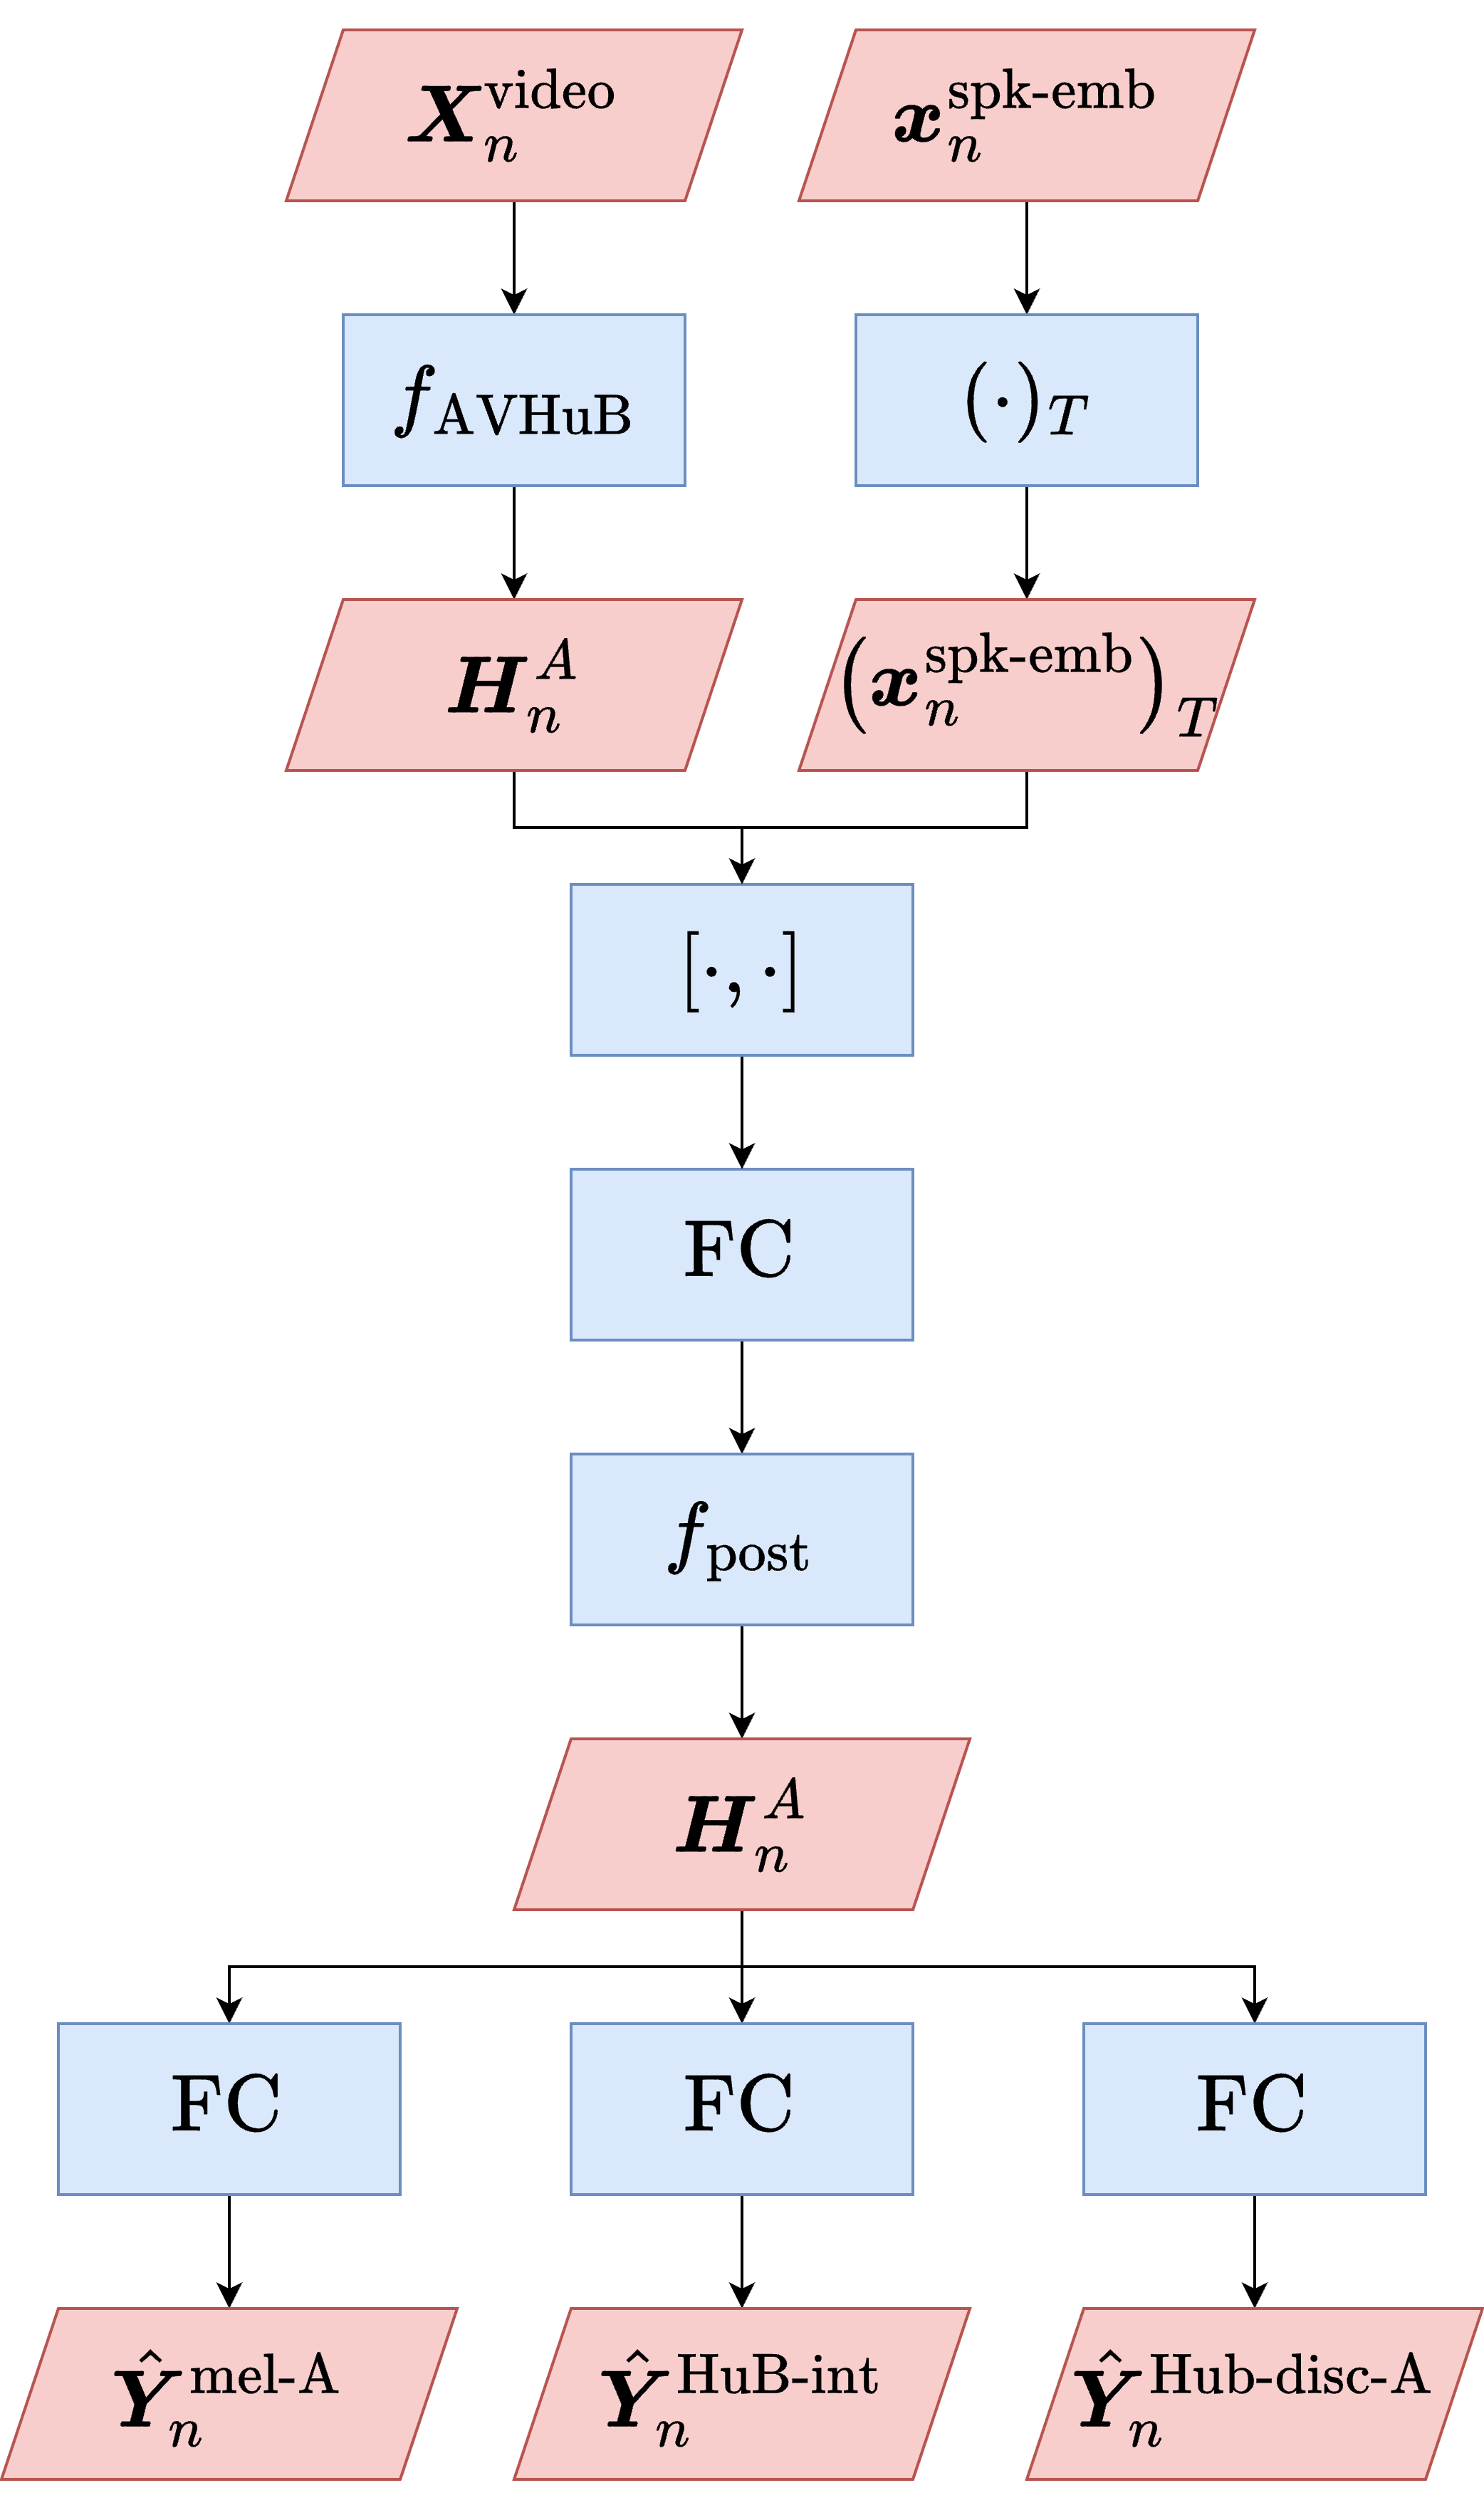
\includegraphics[height=140mm]{./figure/sec4/model_2/networkA.drawio.png}
    \caption{提案手法: ネットワークA}
    \label{sec4:fig:networkA}
\end{figure}

\begin{figure}[tb]
    \centering
    \begin{subfigure}[b]{0.32\textwidth}
        \centering
        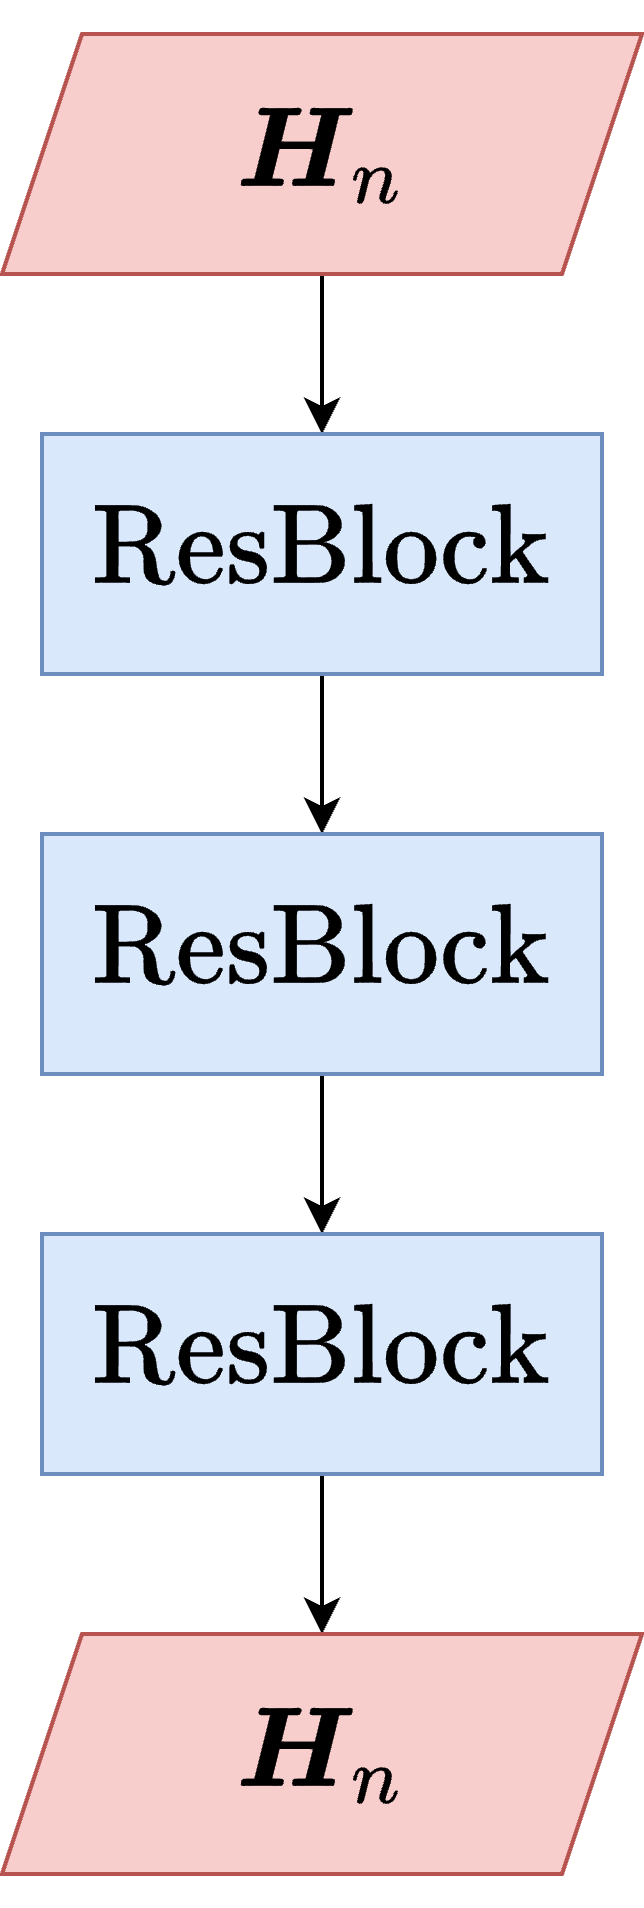
\includegraphics[height=90mm]{./figure/sec4/model_2/post.drawio.png}
        \caption{$\myNetworkPost$の構造}
        \label{sec4:fig:post}
    \end{subfigure}
    \hfill
    \begin{subfigure}[b]{0.32\textwidth}
        \centering
        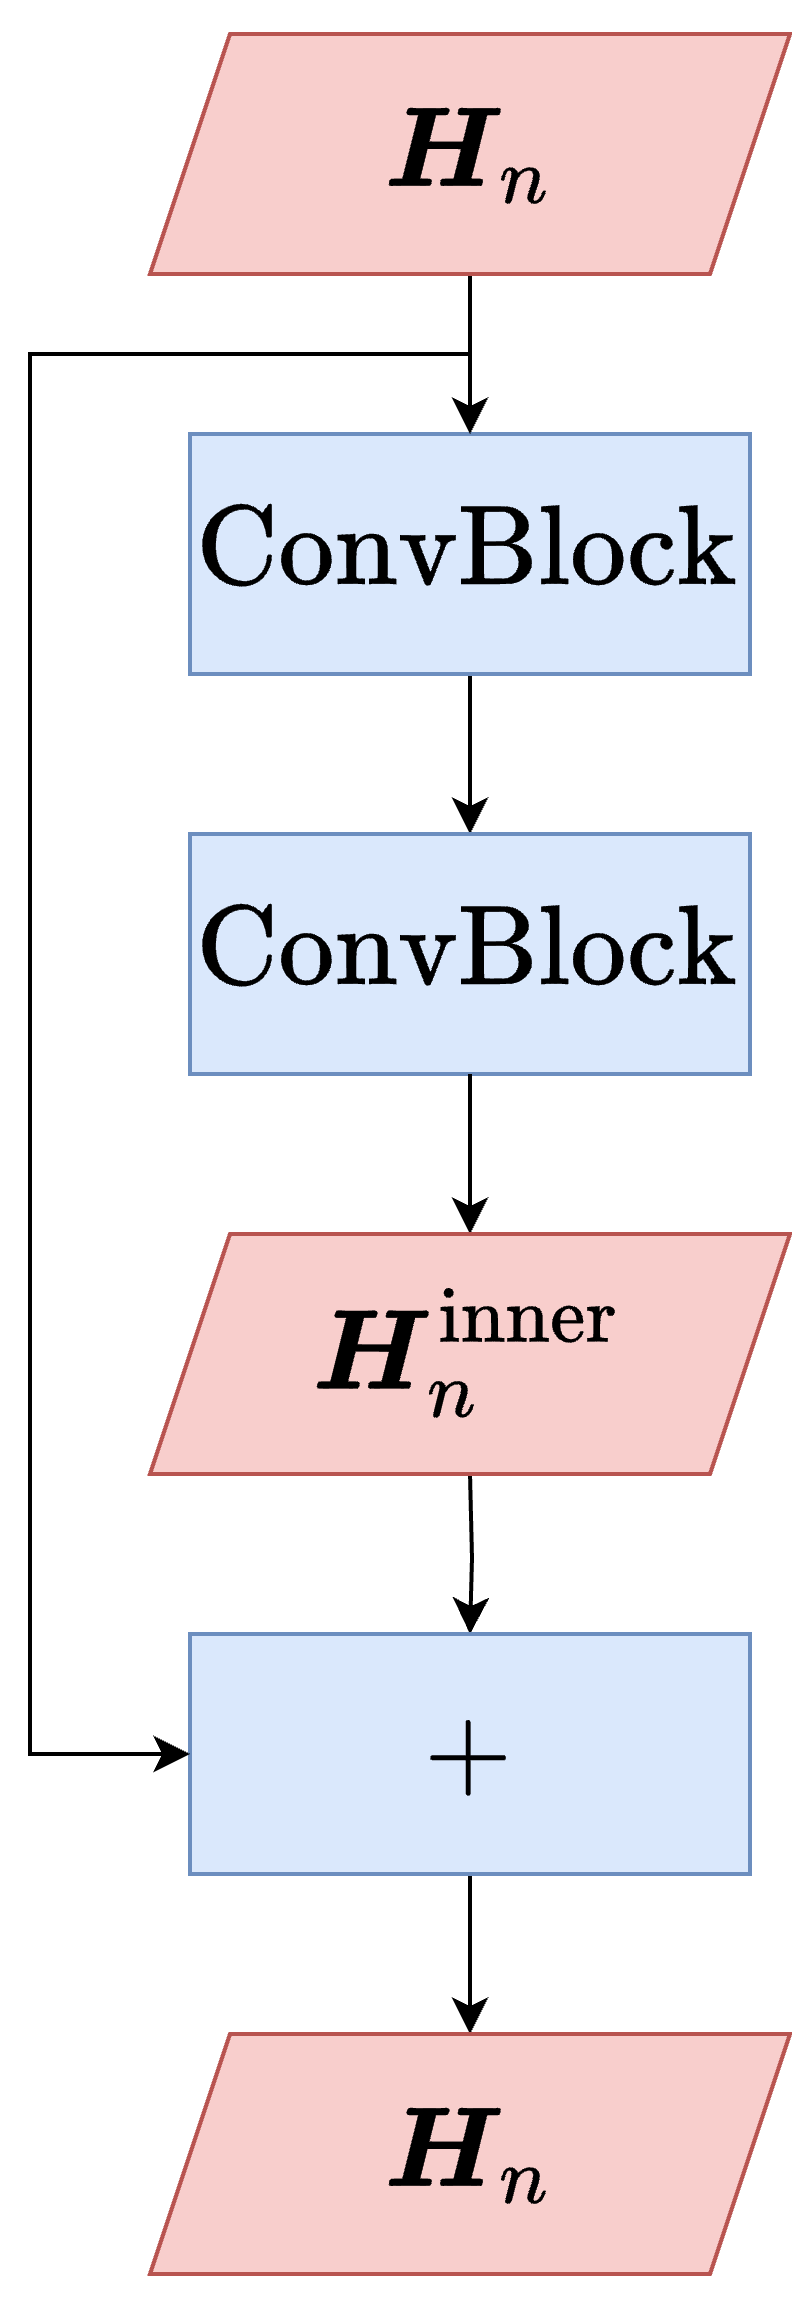
\includegraphics[height=90mm]{./figure/sec4/model_2/post_resblock.drawio.png}
        \caption{$\text{ResBlock}$の構造}
        \label{sec4:fig:post_resblock}
    \end{subfigure}
    \hfill
    \begin{subfigure}[b]{0.32\textwidth}
        \centering
        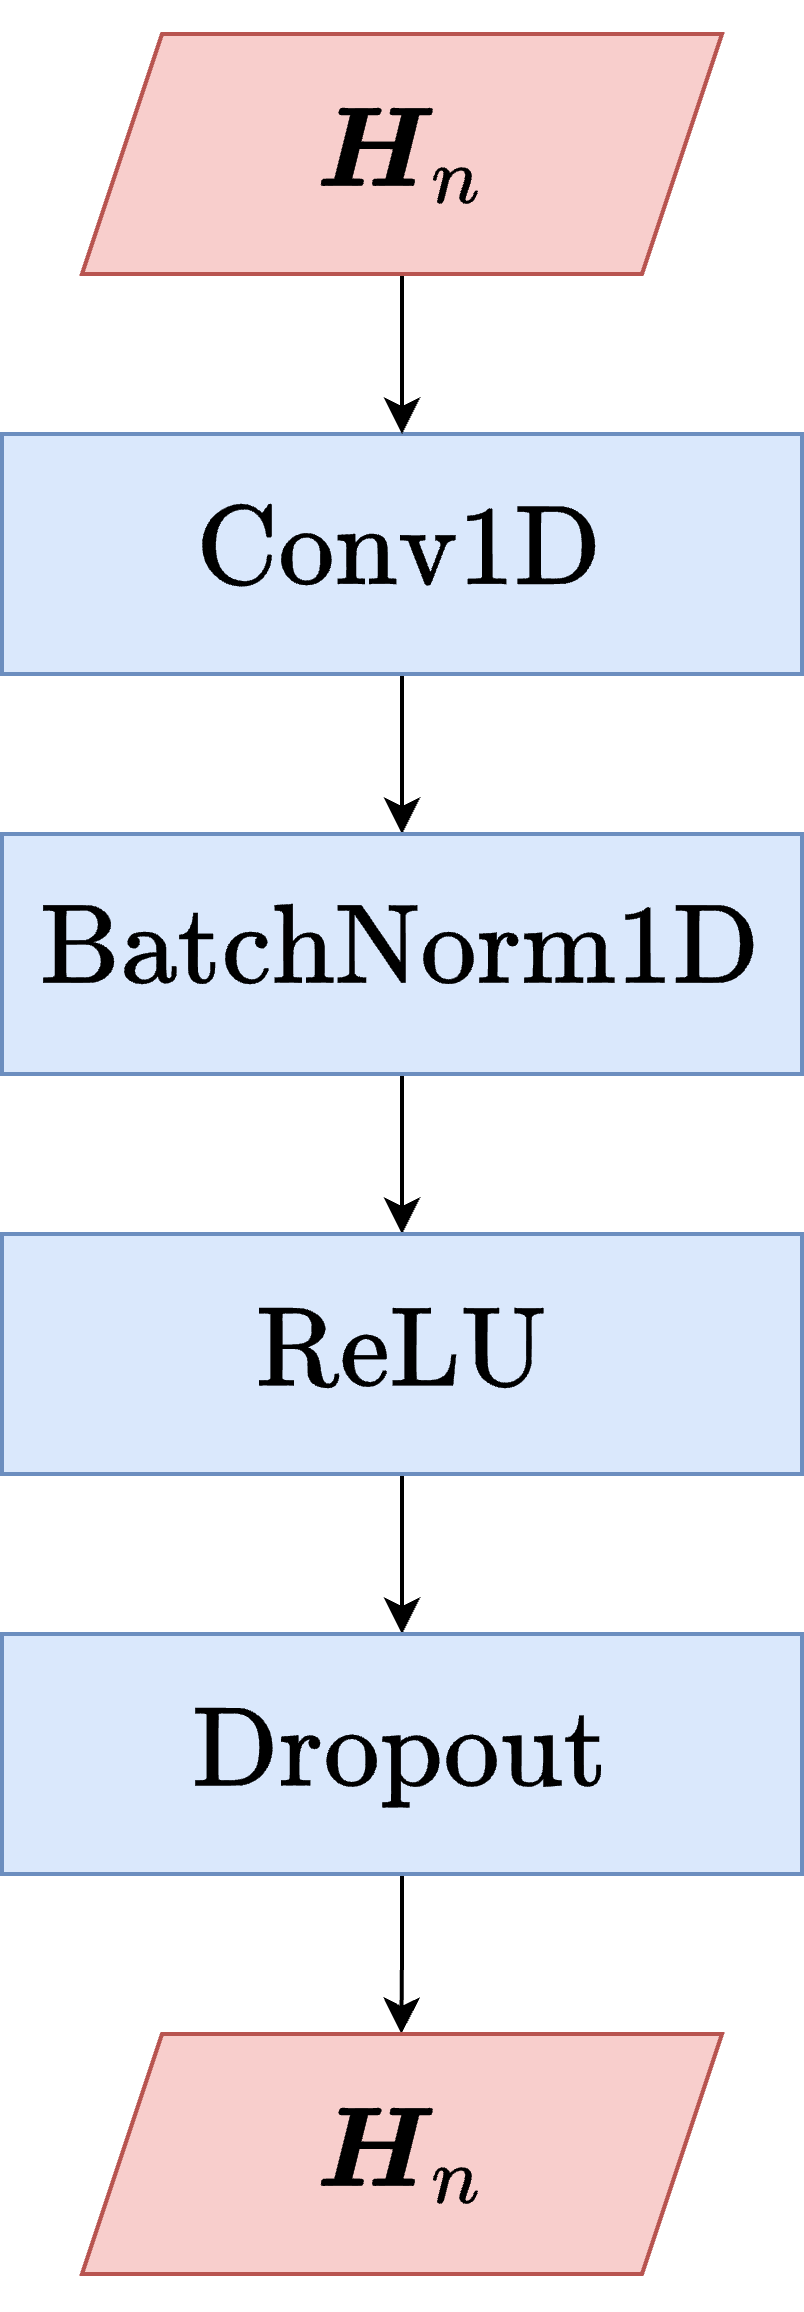
\includegraphics[height=90mm]{./figure/sec4/model_2/post_convblock.drawio.png}
        \caption{$\text{ConvBlock}$の構造}
        \label{sec4:fig:post_convblock}
    \end{subfigure}
    \caption{提案手法: 後処理層$\myNetworkPost$}
    \label{sec4:fig:post_three_step}
\end{figure}

\subsubsection{ネットワークB}
ネットワークBを図\ref{sec4:fig:networkB}に示す。ネットワークBでは,まず,ネットワークAで得られた予測HuBERT中間特徴量$\hubertIntPred$を$\hubertTransformer$に通すことで,特徴量$\featureB \in \featureBSet$に変換する.これは,
\begin{equation}
    \featureB = \hubertTransformer\lr{\hubertIntPred; \weightB}
\end{equation}
と表される.以下,ネットワークAと処理は同様であるため,数式のみ記載する.
\begin{gather}
    \featureB = \myNetworkSpkMerge\lr{\concat{\featureB, \lrRepeat{\spkEmb}{T}}; \weightB} \\
    \featureB = \myNetworkPost\lr{\featureB; \weightB} \\
    \melPredB = \myNetworkFcMel\lr{\featureB; \weightB} \\
    \hubertDiscPredB = \myNetworkFcHubDisc\lr{\featureB; \weightB}
\end{gather}

ネットワークBの役割は,メルスペクトログラムとHuBERT離散特徴量の予測である.HuBERT Transformer層の転移学習を検討した狙いは、HuBERTの自己教師あり学習の方法に基づく。HuBERTはMasked Predictionという自己教師あり学習を行っており、これは、畳み込みエンコーダ$\hubertConv$からの出力にマスクを適用し,Transformer層$\hubertTransformer$を通すことによって、マスクされた部分を推定する学習方法である.\ref{sec3:sec:ssl}節より、Masked Predictionでは未知の情報を正しく穴埋めできるように観測できる情報から特徴抽出を行う必要があるから,最適化されたHuBERTは音声の文脈的な構造を学習していると考えられる.また、Masked Predictionは音声データのみによる学習が可能であり、近年では大規模なデータによって学習されたモデルも一般に公開されている。よって、本研究ではHuBERT Transformer層を動画音声合成にFine Tuningすることにより,動画を入力とするネットワークAにおける推定残差を,大量の音声データから学習された音声自体の文脈を考慮する力によって軽減することで、最終予測値であるメルスペクトログラムとHuBERT離散特徴量に対する推定精度改善を狙った.

\begin{figure}[bt]
    \centering
    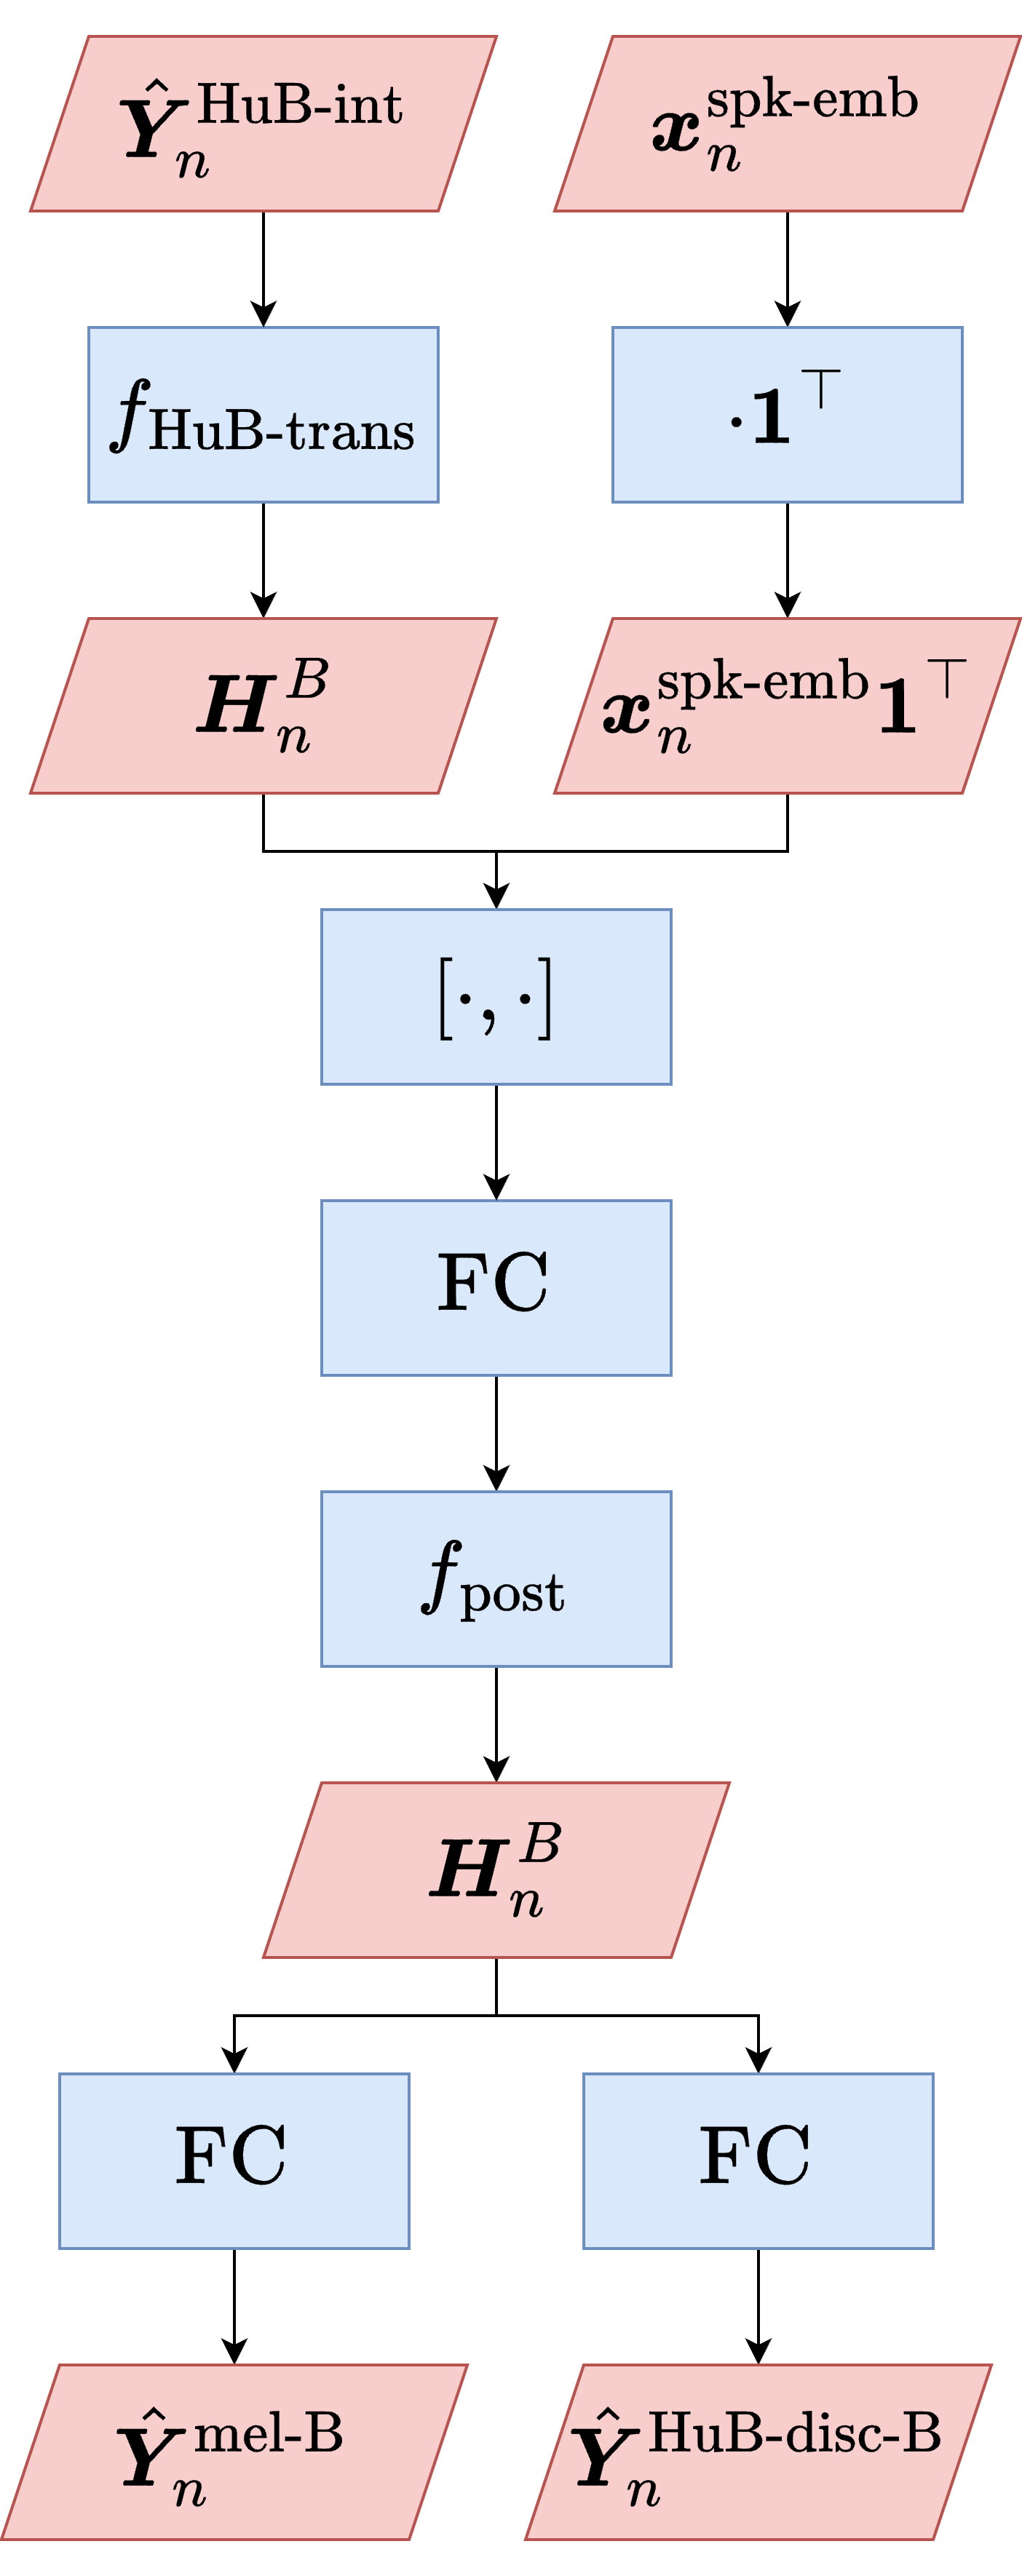
\includegraphics[height=140mm]{./figure/sec4/model_2/networkB.drawio.png}
    \caption{提案手法: ネットワークB}
    \label{sec4:fig:networkB}
\end{figure}

\subsubsection{ボコーダ}
ボコーダを図\ref{sec4:fig:vocoder}に示す。本実験で用いるボコーダは、今回ベースラインとする先行研究\cite{choi2023intelligible}で提案されたMulti-input Vocoderを参考にしたものである。まず,ネットワークBで得られた予測メルスペクトログラム$\melPredB$とHuBERT離散特徴量に対するロジット$\hubertDiscPredB$を前処理層に通し,扱いやすい形状に変換する.これは,
\begin{gather}
    \featureVocMel = \vocoderPreMel\lr{\melPredB; \weightVoc} \\
    \featureVocHuBERT = \vocoderPreHub\lr{\hubertDiscPredB; \weightVoc}
\end{gather}
と表される.$\featureVocMel \in \featureVocMelSet$は,$\melPredB$の時間方向に隣接したベクトルを次元方向に結合することで$\hubertDiscPredB$と系列長を揃え、その後全結合層を適用した特徴量である.一方,$\featureVocHuBERT \in \featureVocHuBERTSet$は,$\hubertDiscPredB$に対して$\argmax$関数を適用した後,各時刻$t$において選択されたインデックスをベクトルに変換した特徴量である.次に,$\featureVocMel, \featureVocHuBERT$を入力として,音声波形を生成する.これは,
\begin{equation}
    \spWaveformPred = \vocoderMain\lr{\concat{\featureVocMel, \featureVocHuBERT}; \weightVoc}
\end{equation}
と表される.$\vocoderMain$の具体的な処理はHiFi-GANのGeneratorと同様であり,本実験ではボコーダ自体ではなく,ボコーダ入力を予測する手法の検討に焦点を当てたから,ここでは詳細は割愛する.

\begin{figure}[bt]
    \centering
    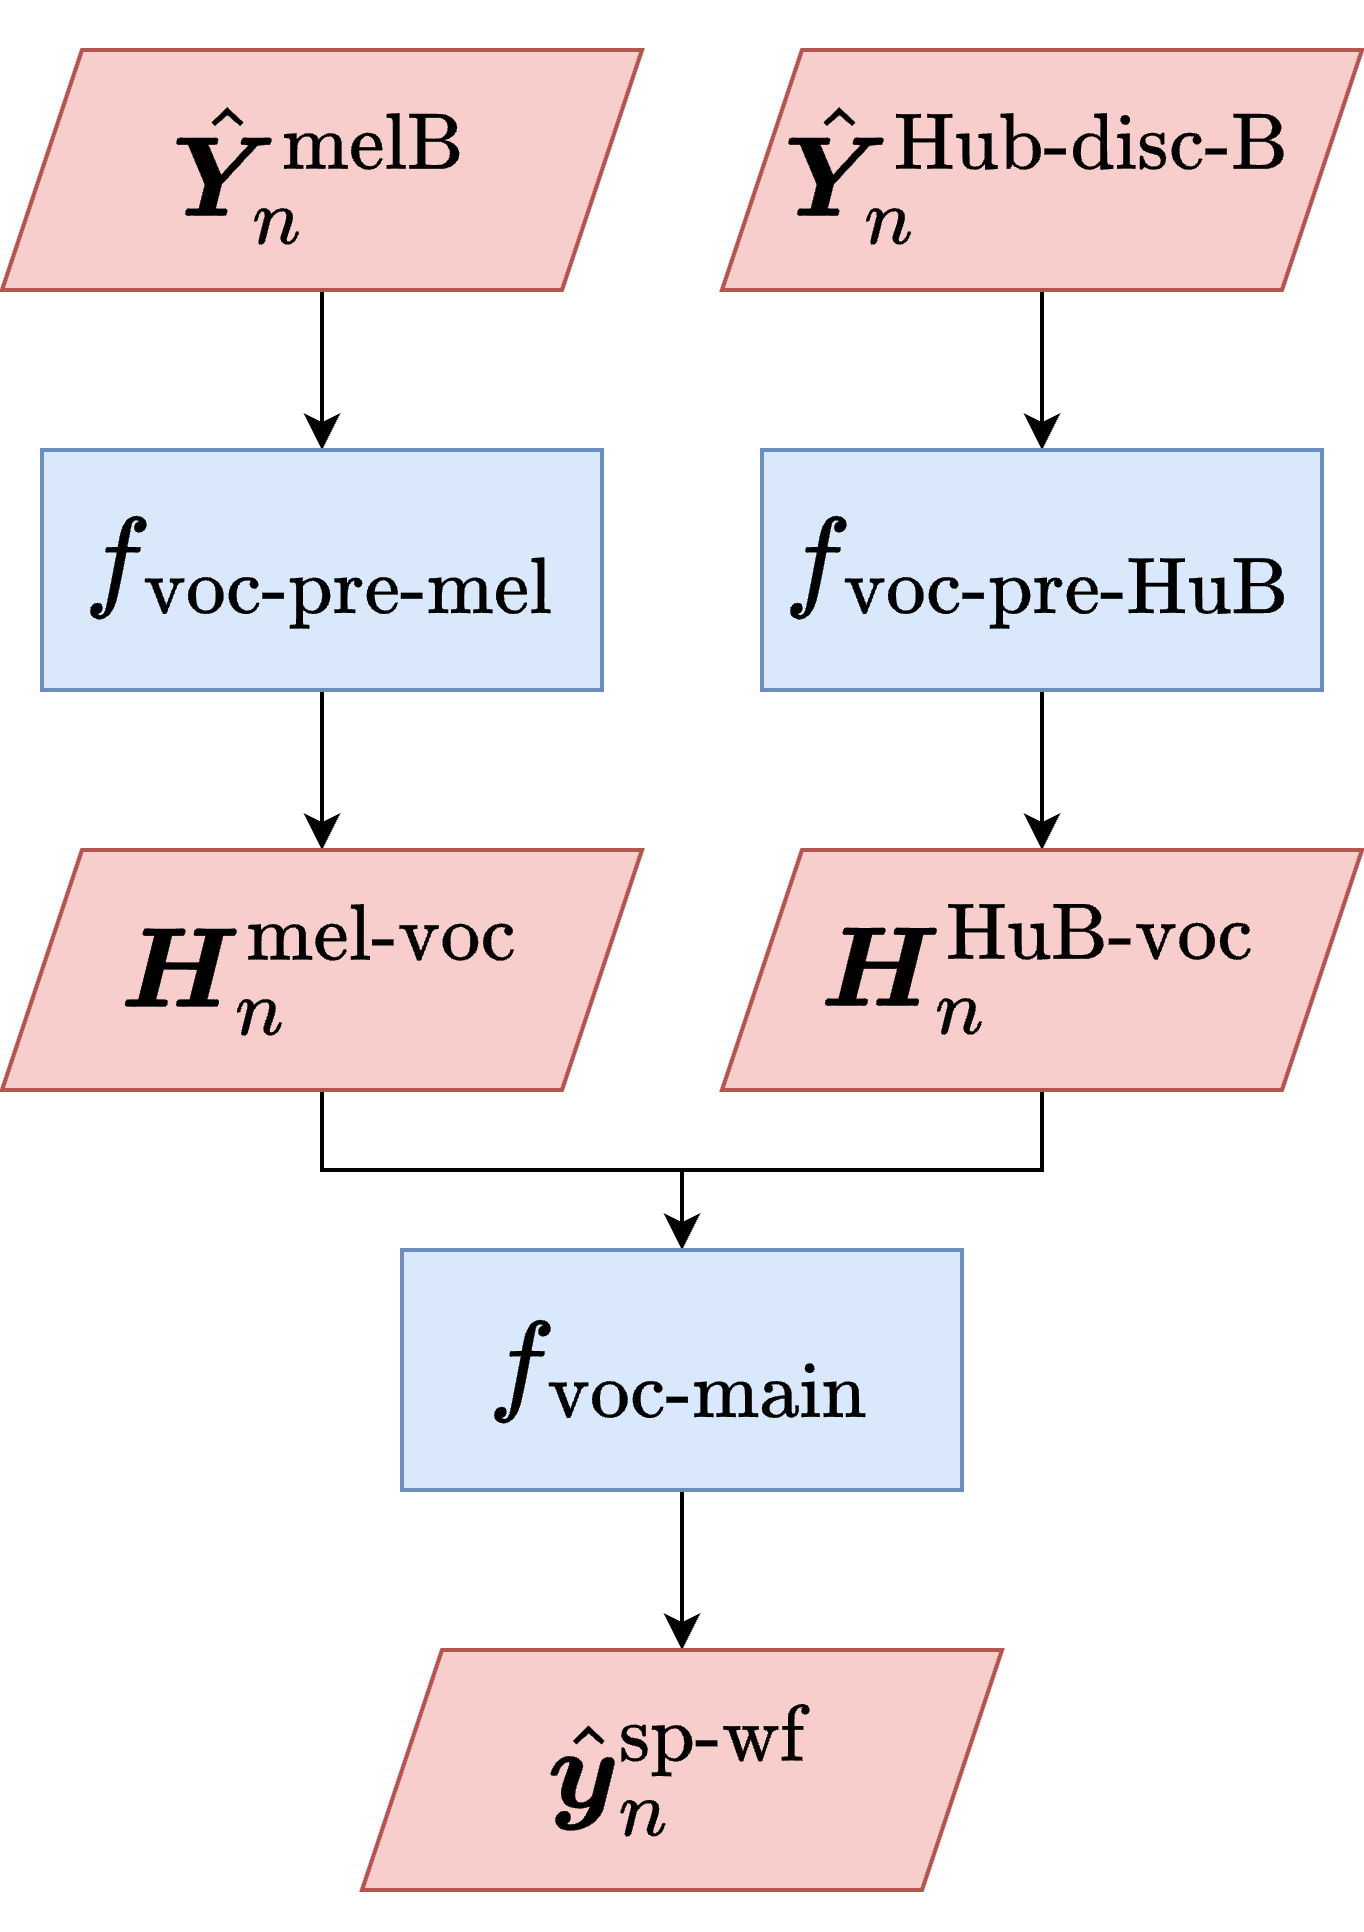
\includegraphics[height=80mm]{./figure/sec4/model_2/vocoder.drawio.png}
    \caption{提案手法: ボコーダ}
    \label{sec4:fig:vocoder}
\end{figure}

\subsubsection{損失関数}
まず,ネットワークAの学習に用いる損失関数$\lossFuncUpper_{A}$は,
\begin{equation}
    \begin{aligned}
        \lossFuncUpper_{A} & \lr{\hubertIntGt, \hubertIntPred, \melGt, \melPredA, \hubertDiscGt, \hubertDiscPredA}                 \\
        =                  & \lossWeightHubInt \lossMAE{\hubertIntGt}{\hubertIntPred} + \lossWeightMel \lossMAE{\melGt}{\melPredA} \\
                           & + \lossWeightHubDisc \lossCE{\hubertDiscGt}{\hubertDiscPredA}
    \end{aligned}
\end{equation}
で与えられる.すなわち,HuBERT中間特徴量とメルスペクトログラムについてのMAE Loss,HuBERT離散特徴量についてのCross Entropy Lossの重み付け和である.次に,ネットワークBの学習に用いる損失関数$\lossFuncUpper_{B}$は,
\begin{equation}
    \begin{aligned}
        \lossFuncUpper_{B} & \lr{\melGt, \melPredB, \hubertDiscGt, \hubertDiscPredB}                                                  \\
        =                  & \lossWeightMel \lossMAE{\melGt}{\melPredB} + \lossWeightHubDisc \lossCE{\hubertDiscGt}{\hubertDiscPredB}
    \end{aligned}
\end{equation}
で与えられる.すなわち,メルスペクトログラムについてのMAE Loss,HuBERT離散特徴量についてのCross Entropy Lossの重み付け和である.最後に,ボコーダの学習に用いる損失関数について,これはHiFi-GANと同様であるから,ここでは割愛する.